\documentclass[11pt]{article}
\usepackage{indentfirst}
\usepackage{amsmath}
%\usepackage{a4wide} %Wider text on A4 paper
\usepackage[a4paper,includeheadfoot,margin=2cm]{geometry}
\usepackage{graphicx}
\graphicspath{ {/Report/} } % we have to call pdflatex from the folder above /Report
                            % to make sure pdflatex can find the images

\title{SWEN90004 Modelling Complex Software System\\
        \textbf{Assignment 2 Report}}
\author{Zheping Liu, 683781, zhepingl\\
        Zewen Xu, 862393, zewenx}
\date{}

%TODO: This is a comment in Latex

\begin{document}
    \maketitle
    \section{Background}
        The chosen model for our analysis is the \textbf{Rebellion} model. 
        This model is based on model of civil violence by Joshua Epstein (2002).
        The aim of this project is to replicate this model and study how this 
        complex system behaves in different stages and under different settings.
        It describes the how agents behave against central authority in relation
        to their grievance and the power of authority.
        \paragraph{}
        \textbf{Rebellion} is a complex system. Firstly, this model is made
        of many individual instances, each of them has individual state, but at
        the same time, their behaviour (i.e. state transitions) are affected by
        other states of other instances near them. Secondly, the states of the 
        whole system is unpredictable at a certain time t with a given set of inputs.
        This is due to the interrelation and interactions between states of 
        different instances and certain degree of randomness in this model. 
        Thirdly, under most settings, the model is decentralised. The vision of
        most instances cannot cover the whole board. Also, all agents are the same, 
        and all cops are the same, none of them is a leader in this model. This
        implies they all contribute the same amount to influence the states of the
        model. Fourthly, there is feedback on the behaviour of agents. Active agents
        can eventually influence agents around them and lead to more active agents.
        Also, more active agents will attract more cops to enforce on them, which
        leads to more quiet agents. Finally, although there exists regular patterns 
        for states of the system, but it does not approach to an equilibrium. 
        
    \section{Model}
        The model includes the following major components:
        \subsection{Board}
        Board is the representation of the world in this model. It is set in default
        to contain $1600\:(40 \times 40)$ patches in total.
        \subsubsection{Patches}
        Each patch in the board has two states, \textit{empty} and \textit{occupied}.
        \subsection{Agent}
        Agents are the representation of ordinary individuals in this model. Agents
        have three states, \textit{active}, \textit{quiet} and \textit{jailed}. 
        They are default to be \textit{quiet} at the beginning. Agents will be able
        to move to any empty patches in their vision when \textit{MOVEMENT} value
        equals to \textit{true} every tick. They will update their state after the
        movement phase according to the following equation.
        \begin{equation}
            \begin{split}
                grievance\:-\:riskAversion\:\times\:estimatedArrestProbability\:>\:threshold \\
                \text{Where}\ grievance\:=\:perceivedHardship\:\times\:(1\:-\:governmentLegitimacy)\\
                \text{and}\ estimatedArrestProbability = 1 - e^{-k \times ((1 + activeCount) / copsCount)}
            \end{split}
        \end{equation}  
        When this equation holds, their state will become \textit{active}, otherwise
        it will be \textit{quiet}. Both the number of active agents and number of
        cops around them will be factors that decide their behaviours.
        If active agents are in the vision of cops, there
        will be possibility for them to become \textit{jailed} by the enforce action
        of cops. A random jail term between 0 and the maximum jail term allowed will
        be given to them and they are not able to move or action during that time.
        \subsection{Cop}
        Cops are the representation of power of authority in this model. Cops
        are always allowed to move to empty patches within their vision at 
        every tick. They can enforce at most one active agent within their vision
        at each tick and move to their patches.

    
    \section{Assumptions}
        During replicating the Rebellion model, we have made some assumptions about
        it.
        \paragraph{First assumption} A single patch is able to hold multiple
        characters (includes both \textbf{Agent} and \textbf{Cop}). This assumption
        is made because of patches containing jailed agents are also considered
        as \textit{empty}. Therefore, there is possibility that when jailed agents
        are released and placed back to their previous patches, there are other 
        characters on those patches.
        \paragraph{Second assumption} Characters update their every behaviour (including
        movement, determine behaviour and enforce) in random orders. The NetLogo
        model does not specify the order of characters during each updating phase.
        However, when we are updating characters without random orders, we obtain
        different patterns from the NetLogo results. The status of the model will
        approach equilibrium instead of performing random walk in the later stages 
        under some settings.

    \section{Replication \& Results Analysis}
    \subsection{Scenario 1}
     \begin{table}[ht]
        \begin{center}
          \begin{tabular}{|l|l|}
          \hline
            Initial cop density & 0.04 \\
          \hline
            Initial agent density & 0.70 \\
          \hline
            Vision & 7 \\
          \hline
            Government Legitimacy & 0.82 \\
          \hline
            Max jail term & 30 \\
          \hline
            Movement & True \\
          \hline
          \end{tabular}
          \caption{Scenario 1}\label{table1}
        \end{center}
      \end{table}
      The first scenario is using the default setting from the model in 
      NetLogo.
      \begin{figure}[h!]
        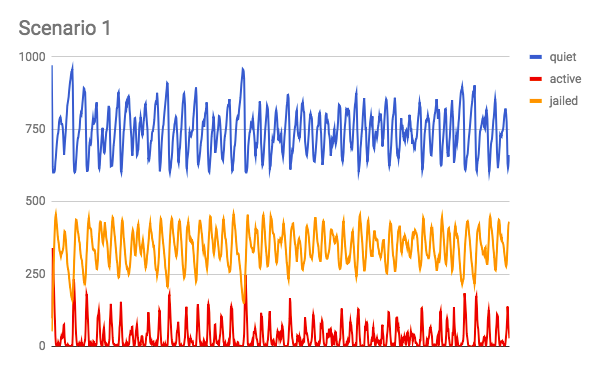
\includegraphics[width=\linewidth]{Scenario_1.png}
        \caption{Scenario 1}
        \label{fig:scenario}
      \end{figure}

      \paragraph{}
      The results of our implementation is very similar to the results of the
      original NetLogo model. 
      \paragraph{}
      They both have similar patterns. With total number
      of active agents increases, the total number of jailed agents will increase
      in next few ticks. This then leads to a decrease in the number of active agents,
      also an increase in the quiet agents. 
      \paragraph{}
      However, there are few differences between these two results. Firstly, the
      average highest number of active agents in the NetLogo model is approximately
      around $300$ to $350$. In our implementation this is only about $200$.
      Secondly, the average highest number of jailed agents in the original model
      is around $400$. In our model it is very close to $500$. The two differences
      above indicates there is stronger central authority in our implementation.
      In other words, the cops are more efficient in our implementation, more
      active agents are arrested.
      %TODO: May illustrate the reason behind this

      \subsection{Scenario 2}
      \begin{table}[ht]
        \begin{center}
          \begin{tabular}{|l|l|}
          \hline
            Initial cop density & 0.04 \\
          \hline
            Initial agent density & \textbf{0.95} \\
          \hline
            Vision & 7 \\
          \hline
            Government Legitimacy & 0.82 \\
          \hline
            Max jail term & 30 \\
          \hline
            Movement & True \\
          \hline
          \end{tabular}
          \caption{Scenario 2}\label{table2}
        \end{center}
      \end{table}
      The second scenario represents when there is only limited space on the board. 
      The initial agent density has been increased to $95\%$, and there is only
      $1\%$ empty spaces left in the board initially.
      \begin{figure}[h!]
        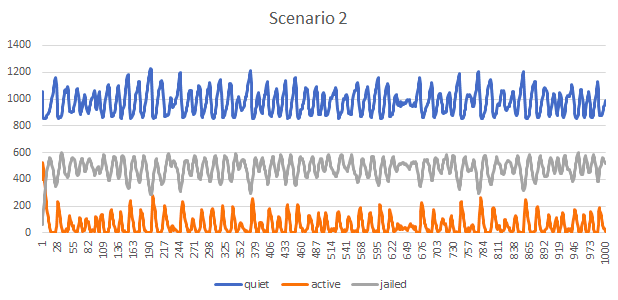
\includegraphics[width=\linewidth]{Scenario_2.png}
        \caption{Scenario 2}
        \label{fig:scenario}
      \end{figure}

      \paragraph{}
      The overall results is very close to the results from the previous setting.
      One difference that can be observed is the ratio of jailed agents comparing
      to the active agents increases. In more detail, the total number of active
      agents remains in the similar level. However, the total number of jailed agents
      has a slight increase, the average highest number of jailed agents is now
      around $600$.
      \paragraph{}
      Nevertheless, in the original NetLogo model, the increase in the number of
      active agents is larger. The average highest number of active agents in the
      original model is $500$, where it is $250$ in our implementation. Also, the
      difference between the number of jailed agents and the number of active agents
      is smaller in the original model. The above difference implies the same conclusion
      as the first scenario, the central authority are more effective in our implemented
      model comparing to the original one.

      \subsection{Scenario 3}
      \begin{table}[ht]
        \begin{center}
          \begin{tabular}{|l|l|}
          \hline
            Initial cop density & 0.04 \\
          \hline
            Initial agent density & 0.70 \\
          \hline
            Vision & 7 \\
          \hline
            Government Legitimacy & \textbf{0.62} \\
          \hline
            Max jail term & 30 \\
          \hline
            Movement & True \\
          \hline
          \end{tabular}
          \caption{Scenario 3}\label{table3}
        \end{center}
      \end{table}
      The government legitimacy is reduced to $0.62$ in this case, the probability
      of agents become \textit{active} increases.
      \begin{figure}[h!]
        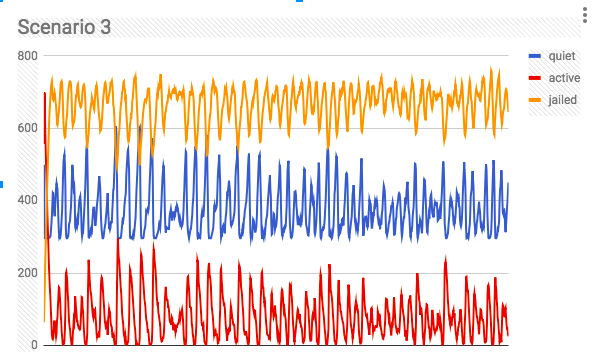
\includegraphics[width=\linewidth]{Scenario_3.png}
        \caption{Scenario 3}
        \label{fig:scenario}
      \end{figure}

      \paragraph{}
      By decreasing the government legitimacy, there is much higher number of 
      jailed agents, even more than the number of quiet agents in our implementation.
      Comparing to jailed agents, the number of active agents remains at the similar
      level compares to \textit{Scenario 1}. This result states that agents are
      more likely to rebel, and then arrested under this scenario.
      \paragraph{}
      Comparing to the original model, this time our implementation has less average
      number of quiet agents. %TODO:

      \subsection{Scenario 4}
      \begin{table}[ht]
        \begin{center}
          \begin{tabular}{|l|l|}
          \hline
            Initial cop density & 0.04 \\
          \hline
            Initial agent density & 0.70 \\
          \hline
            Vision & 7 \\
          \hline
            Government Legitimacy & 0.82 \\
          \hline
            Max jail term & 30 \\
          \hline
            Movement & \textbf{False} \\
          \hline
          \end{tabular}
          \caption{Scenario 4}\label{table4}
        \end{center}
      \end{table}
      In this scenario, the \textit{Movement} is set to \textbf{False}, which is
      only cops are able to move in this case.
      \begin{figure}[h!]
        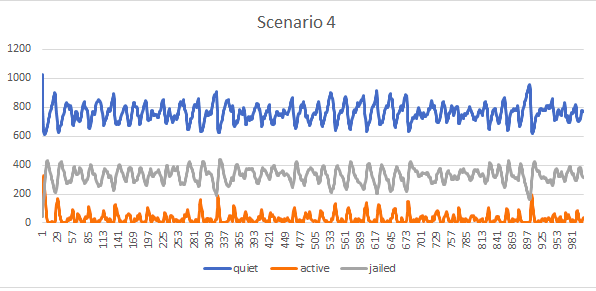
\includegraphics[width=\linewidth]{Scenario_4.png}
        \caption{Scenario 4}
        \label{fig:scenario}
      \end{figure}

      \paragraph{}
      By restricting the move ability of agents, there is less number of active
      agents in our implementation. The reason for this can be agents with higher
      probability to rebel are not able to move together to cause a large rebellion.
      \paragraph{}
      Nevertheless, there is no clear difference when disable the movement in the
      original model. The average highest number of active agents at
      one tick is only around $200$ in our implementation. But it is close to $350$
      in the original NetLogo model. 

      \subsection{Scenario 5}
      \begin{table}[ht]
        \begin{center}
          \begin{tabular}{|l|l|}
          \hline
            Initial cop density & 0.04 \\
          \hline
            Initial agent density & 0.70 \\
          \hline
            Vision & \textbf{5} \\
          \hline
            Government Legitimacy & 0.82 \\
          \hline
            Max jail term & 30 \\
          \hline
            Movement & True \\
          \hline
          \end{tabular}
          \caption{Scenario 5}\label{table5}
        \end{center}
      \end{table}
      The final scenario we have is reducing the \textbf{vision} from 7 to 5.
      \begin{figure}[h!]
        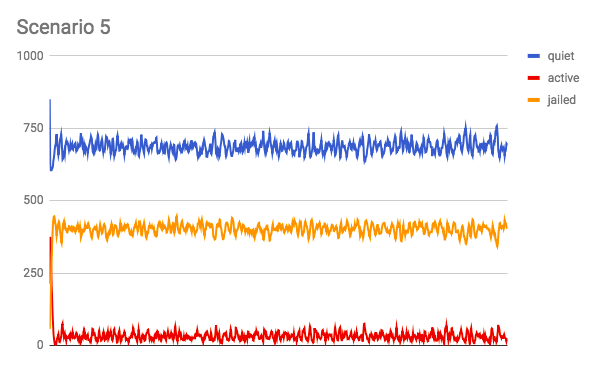
\includegraphics[width=\linewidth]{Scenario_5.png}
        \caption{Scenario 5}
        \label{fig:scenario}
      \end{figure}
      \paragraph{}
      From the above results, there is huge difference between this case and 
      the \textit{Scenario 1}. Firstly, the amplitude of all three lines are much
      smaller than \textit{Scenario 1}. This is since all agents and cops can obtain
      less information than before, therefore, their behaviour is less volatile
      than before. Secondly, the average number of quiet agents slightly decreases
      from $750$ to $700$. Thirdly, the average number of jailed agents increases
      from $350$ to $400$. Finally, the average number of active agents decreases
      from $80$ to around $40$.
      From these three differences, we can conclude that there is slightly increase
      in the number of rebelled agents, and more of them are arrested.
      \paragraph{}
      Under this case, the results of our implementation is very close to the results
      produced by the original model.

    \section{Extension}
        The extension we have implemented is that the government legitimacy will
        increase as the proportion of jailed agents to number of total agents increases.
        The equation we derive is 
        \[GovernmentLegitimacy = \] 
        \begin{flalign}
          \begin{split}
          InitialGovernmentLegitimacy + \frac{JailedAgents}{TotalAgents}
          \times (1 - InitialGovernmentLegitimacy)
          \end{split}
        \end{flalign}
        This extension makes the model more realistic, as the central authority
        gets enforced (more agents are jailed), the government legitimacy increases,
        less agents are willing to rebel. When less people are jailed,
        agents will behave similarly as before.
        \begin{figure}[h!]
          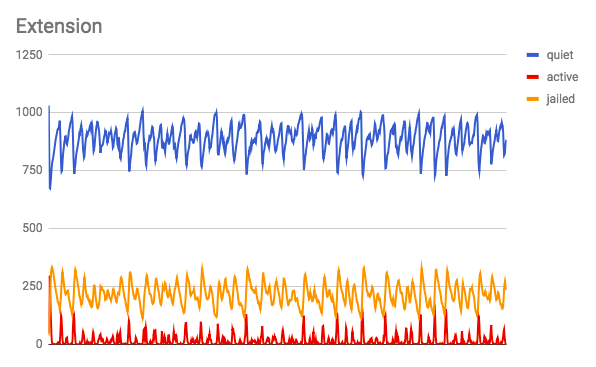
\includegraphics[width=\linewidth]{Extension.png}
          \caption{Extension}
          \label{fig:scenario}
        \end{figure}

        \paragraph{}
        The above chart is the result when applying the extension to the settings
        in \textit{Scenario 1}. Obviously, the average number of quiet agents increases,
        average number of jailed agents and active agents decreases. This proves
        the statement described above. Enforcement will be more effective since it
        not only reduce the number of active agents by putting them in jail, it also
        increases government legitimacy to make less people willing to rebel.

    \section{Conclusion}
    In conclusion, we have done five experiments under different parameters. To
    observe the effect of each parameter, each of the later four scenarios only modifies
    one parameter from the base case, that is, \textit{Scenario 1}. Parameters such as
    \textbf{government legitimacy} and \textbf{vision} are very effective to the
    model. Other parameters such as \textbf{agent-density} and \textbf{movement}
    only have limited effect on the model by themselves. In addition, there is
    some differentiation between the model we implement and the original NetLogo
    model, like more effective cops during enforce phase. 

    \newpage

    \section{Appendix}
    When we first tried to start designing the Java implementation, we found
    some specification of the model was missing.
    As a result, we extended the model with some new classes. In order to simulate 
    the model with Java, we tried to understand the logic of the model in NetLogo.
    However, the code in NetLogo is not precise. Many conditions are not described 
    clearly in the model, such as the process of moving a character in the board. 
    We tried to figure out how NetLogo moves people on board by reading the official
    documents, but we did not find useful information from them. We finally resolve
    this problem by observing the behaviour of the NetLogo model, and made some
    assumptions, we even developed more than one version of code to experiment the
    true logic behind these hidden functions.
    After we finished the first version, we found that our java model behaves quite differently
    from the original model. We had to read through our codes to fix the incorrect
    behaviour of model. Nevertheless, currently there are still few inconsistent
    behaviours between our implementation and the original model. We have identified
    them in the report.
    To make the structure and design of our implementation more clear, we refactored
    our code after most bugs are fixed. 
    
\end{document}